\documentclass[1p]{elsarticle_modified}
%\bibliographystyle{elsarticle-num}

%\usepackage[colorlinks]{hyperref}
%\usepackage{abbrmath_seonhwa} %\Abb, \Ascr, \Acal ,\Abf, \Afrak
\usepackage{amsfonts}
\usepackage{amssymb}
\usepackage{amsmath}
\usepackage{amsthm}
\usepackage{scalefnt}
\usepackage{amsbsy}
\usepackage{kotex}
\usepackage{caption}
\usepackage{subfig}
\usepackage{color}
\usepackage{graphicx}
\usepackage{xcolor} %% white, black, red, green, blue, cyan, magenta, yellow
\usepackage{float}
\usepackage{setspace}
\usepackage{hyperref}

\usepackage{tikz}
\usetikzlibrary{arrows}

\usepackage{multirow}
\usepackage{array} % fixed length table
\usepackage{hhline}

%%%%%%%%%%%%%%%%%%%%%
\makeatletter
\renewcommand*\env@matrix[1][\arraystretch]{%
	\edef\arraystretch{#1}%
	\hskip -\arraycolsep
	\let\@ifnextchar\new@ifnextchar
	\array{*\c@MaxMatrixCols c}}
\makeatother %https://tex.stackexchange.com/questions/14071/how-can-i-increase-the-line-spacing-in-a-matrix
%%%%%%%%%%%%%%%

\usepackage[normalem]{ulem}

\newcommand{\msout}[1]{\ifmmode\text{\sout{\ensuremath{#1}}}\else\sout{#1}\fi}
%SOURCE: \msout is \stkout macro in https://tex.stackexchange.com/questions/20609/strikeout-in-math-mode

\newcommand{\cancel}[1]{
	\ifmmode
	{\color{red}\msout{#1}}
	\else
	{\color{red}\sout{#1}}
	\fi
}

\newcommand{\add}[1]{
	{\color{blue}\uwave{#1}}
}

\newcommand{\replace}[2]{
	\ifmmode
	{\color{red}\msout{#1}}{\color{blue}\uwave{#2}}
	\else
	{\color{red}\sout{#1}}{\color{blue}\uwave{#2}}
	\fi
}

\newcommand{\Sol}{\mathcal{S}} %segment
\newcommand{\D}{D} %diagram
\newcommand{\A}{\mathcal{A}} %arc


%%%%%%%%%%%%%%%%%%%%%%%%%%%%%5 test

\def\sl{\operatorname{\textup{SL}}(2,\Cbb)}
\def\psl{\operatorname{\textup{PSL}}(2,\Cbb)}
\def\quan{\mkern 1mu \triangleright \mkern 1mu}

\theoremstyle{definition}
\newtheorem{thm}{Theorem}[section]
\newtheorem{prop}[thm]{Proposition}
\newtheorem{lem}[thm]{Lemma}
\newtheorem{ques}[thm]{Question}
\newtheorem{cor}[thm]{Corollary}
\newtheorem{defn}[thm]{Definition}
\newtheorem{exam}[thm]{Example}
\newtheorem{rmk}[thm]{Remark}
\newtheorem{alg}[thm]{Algorithm}

\newcommand{\I}{\sqrt{-1}}
\begin{document}

%\begin{frontmatter}
%
%\title{Boundary parabolic representations of knots up to 8 crossings}
%
%%% Group authors per affiliation:
%\author{Yunhi Cho} 
%\address{Department of Mathematics, University of Seoul, Seoul, Korea}
%\ead{yhcho@uos.ac.kr}
%
%
%\author{Seonhwa Kim} %\fnref{s_kim}}
%\address{Center for Geometry and Physics, Institute for Basic Science, Pohang, 37673, Korea}
%\ead{ryeona17@ibs.re.kr}
%
%\author{Hyuk Kim}
%\address{Department of Mathematical Sciences, Seoul National University, Seoul 08826, Korea}
%\ead{hyukkim@snu.ac.kr}
%
%\author{Seokbeom Yoon}
%\address{Department of Mathematical Sciences, Seoul National University, Seoul, 08826,  Korea}
%\ead{sbyoon15@snu.ac.kr}
%
%\begin{abstract}
%We find all boundary parabolic representation of knots up to 8 crossings.
%
%\end{abstract}
%\begin{keyword}
%    \MSC[2010] 57M25 
%\end{keyword}
%
%\end{frontmatter}

%\linenumbers
%\tableofcontents
%
\newcommand\colored[1]{\textcolor{white}{\rule[-0.35ex]{0.8em}{1.4ex}}\kern-0.8em\color{red} #1}%
%\newcommand\colored[1]{\textcolor{white}{ #1}\kern-2.17ex	\textcolor{white}{ #1}\kern-1.81ex	\textcolor{white}{ #1}\kern-2.15ex\color{red}#1	}

{\Large $\underline{12n_{0389}~(K12n_{0389})}$}

\setlength{\tabcolsep}{10pt}
\renewcommand{\arraystretch}{1.6}
\vspace{1cm}\begin{tabular}{m{100pt}>{\centering\arraybackslash}m{274pt}}
\multirow{5}{120pt}{
	\centering
	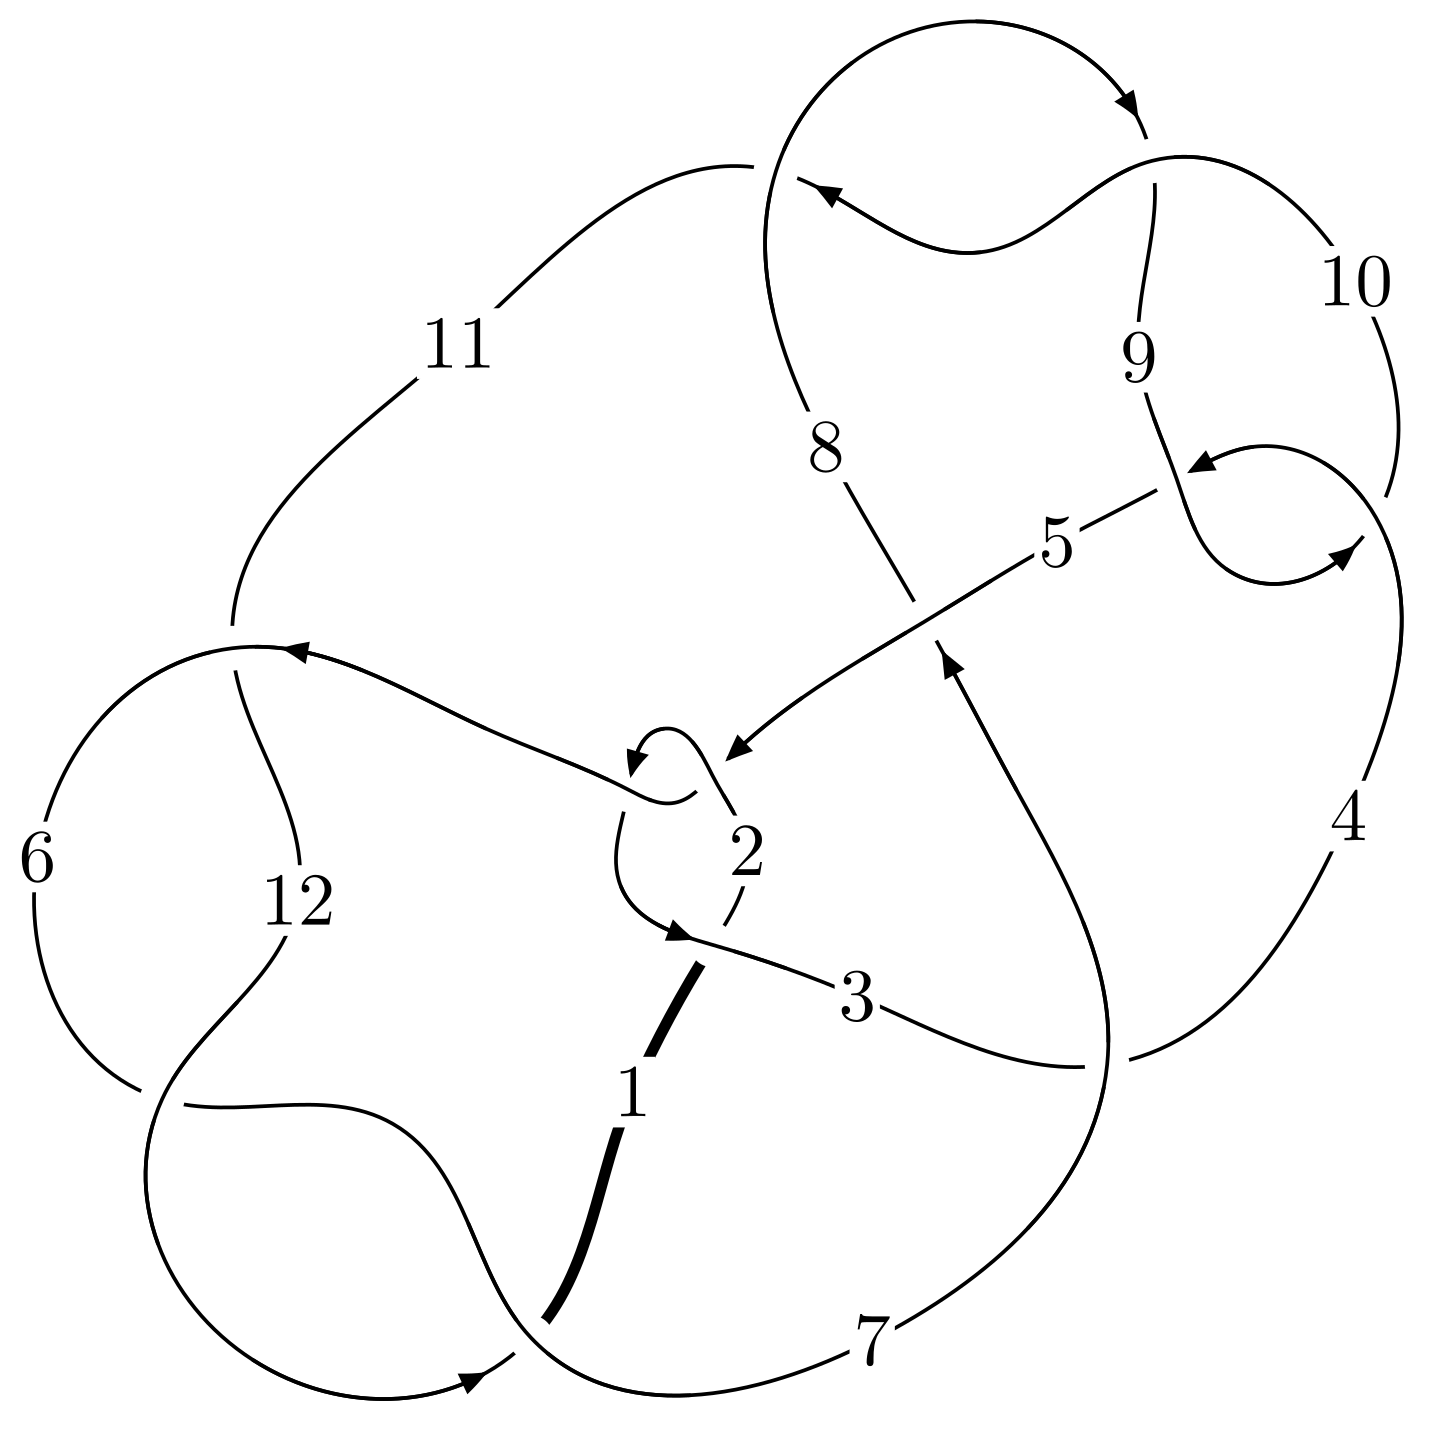
\includegraphics[width=112pt]{../../../GIT/diagram.site/Diagrams/png/2478_12n_0389.png}\\
\ \ \ A knot diagram\footnotemark}&
\allowdisplaybreaks
\textbf{Linearized knot diagam} \\
\cline{2-2}
 &
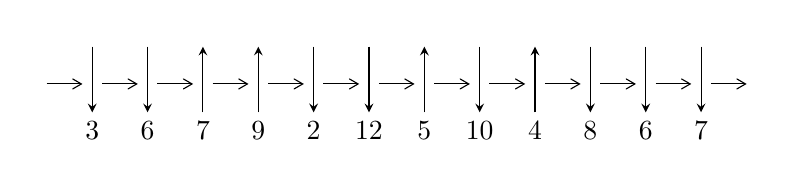
\begin{tikzpicture}[x=20pt, y=17pt]
	% nodes
	\node (C0) at (0, 0) {};
	\node (C1) at (1, 0) {};
	\node (C1U) at (1, +1) {};
	\node (C1D) at (1, -1) {3};

	\node (C2) at (2, 0) {};
	\node (C2U) at (2, +1) {};
	\node (C2D) at (2, -1) {6};

	\node (C3) at (3, 0) {};
	\node (C3U) at (3, +1) {};
	\node (C3D) at (3, -1) {7};

	\node (C4) at (4, 0) {};
	\node (C4U) at (4, +1) {};
	\node (C4D) at (4, -1) {9};

	\node (C5) at (5, 0) {};
	\node (C5U) at (5, +1) {};
	\node (C5D) at (5, -1) {2};

	\node (C6) at (6, 0) {};
	\node (C6U) at (6, +1) {};
	\node (C6D) at (6, -1) {12};

	\node (C7) at (7, 0) {};
	\node (C7U) at (7, +1) {};
	\node (C7D) at (7, -1) {5};

	\node (C8) at (8, 0) {};
	\node (C8U) at (8, +1) {};
	\node (C8D) at (8, -1) {10};

	\node (C9) at (9, 0) {};
	\node (C9U) at (9, +1) {};
	\node (C9D) at (9, -1) {4};

	\node (C10) at (10, 0) {};
	\node (C10U) at (10, +1) {};
	\node (C10D) at (10, -1) {8};

	\node (C11) at (11, 0) {};
	\node (C11U) at (11, +1) {};
	\node (C11D) at (11, -1) {6};

	\node (C12) at (12, 0) {};
	\node (C12U) at (12, +1) {};
	\node (C12D) at (12, -1) {7};
	\node (C13) at (13, 0) {};

	% arrows
	\draw[->,>={angle 60}]
	(C0) edge (C1) (C1) edge (C2) (C2) edge (C3) (C3) edge (C4) (C4) edge (C5) (C5) edge (C6) (C6) edge (C7) (C7) edge (C8) (C8) edge (C9) (C9) edge (C10) (C10) edge (C11) (C11) edge (C12) (C12) edge (C13) ;	\draw[->,>=stealth]
	(C1U) edge (C1D) (C2U) edge (C2D) (C3D) edge (C3U) (C4D) edge (C4U) (C5U) edge (C5D) (C6U) edge (C6D) (C7D) edge (C7U) (C8U) edge (C8D) (C9D) edge (C9U) (C10U) edge (C10D) (C11U) edge (C11D) (C12U) edge (C12D) ;
	\end{tikzpicture} \\
\hhline{~~} \\& 
\textbf{Solving Sequence} \\ \cline{2-2} 
 &
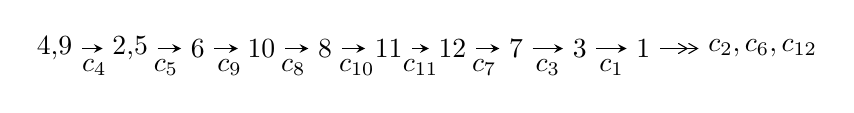
\begin{tikzpicture}[x=23pt, y=7pt]
	% node
	\node (A0) at (-1/8, 0) {4,9};
	\node (A1) at (17/16, 0) {2,5};
	\node (A2) at (17/8, 0) {6};
	\node (A3) at (25/8, 0) {10};
	\node (A4) at (33/8, 0) {8};
	\node (A5) at (41/8, 0) {11};
	\node (A6) at (49/8, 0) {12};
	\node (A7) at (57/8, 0) {7};
	\node (A8) at (65/8, 0) {3};
	\node (A9) at (73/8, 0) {1};
	\node (C1) at (1/2, -1) {$c_{4}$};
	\node (C2) at (13/8, -1) {$c_{5}$};
	\node (C3) at (21/8, -1) {$c_{9}$};
	\node (C4) at (29/8, -1) {$c_{8}$};
	\node (C5) at (37/8, -1) {$c_{10}$};
	\node (C6) at (45/8, -1) {$c_{11}$};
	\node (C7) at (53/8, -1) {$c_{7}$};
	\node (C8) at (61/8, -1) {$c_{3}$};
	\node (C9) at (69/8, -1) {$c_{1}$};
	\node (A10) at (11, 0) {$c_{2},c_{6},c_{12}$};

	% edge
	\draw[->,>=stealth]	
	(A0) edge (A1) (A1) edge (A2) (A2) edge (A3) (A3) edge (A4) (A4) edge (A5) (A5) edge (A6) (A6) edge (A7) (A7) edge (A8) (A8) edge (A9) ;
	\draw[->>,>={angle 60}]	
	(A9) edge (A10);
\end{tikzpicture} \\ 

\end{tabular} \\

\footnotetext{
The image of knot diagram is generated by the software ``\textbf{Draw programme}" developed by Andrew Bartholomew(\url{http://www.layer8.co.uk/maths/draw/index.htm\#Running-draw}), where we modified some parts for our purpose(\url{https://github.com/CATsTAILs/LinksPainter}).
}\phantom \\ \newline 
\centering \textbf{Ideals for irreducible components\footnotemark of $X_{\text{par}}$} 
 
\begin{align*}
I^u_{1}&=\langle 
- u^{27}-2 u^{26}+\cdots+b-1,\;u^{27}+u^{26}+\cdots+2 a-2,\;u^{28}+3 u^{27}+\cdots+2 u+2\rangle \\
I^u_{2}&=\langle 
- u^{15} a+u^{15}+\cdots- a+3,\;-2 u^{15} a+2 u^{15}+\cdots-2 a+2,\\
\phantom{I^u_{2}}&\phantom{= \langle  }u^{16}- u^{15}+3 u^{14}-2 u^{13}+7 u^{12}-4 u^{11}+10 u^{10}-4 u^9+11 u^8-2 u^7+8 u^6+4 u^4+2 u^3+2 u-1\rangle \\
I^u_{3}&=\langle 
- u^2+b- u+1,\;- u^3+2 u^2+2 a- u+4,\;u^4+u^2+2\rangle \\
I^u_{4}&=\langle 
b+u+2,\;a+u+3,\;u^2+1\rangle \\
I^u_{5}&=\langle 
u^3+u^2+b+1,\;a- u-1,\;u^4+1\rangle \\
\\
I^v_{1}&=\langle 
a,\;b+1,\;v+1\rangle \\
\end{align*}
\raggedright * 6 irreducible components of $\dim_{\mathbb{C}}=0$, with total 71 representations.\\
\footnotetext{All coefficients of polynomials are rational numbers. But the coefficients are sometimes approximated in decimal forms when there is not enough margin.}
\newpage
\renewcommand{\arraystretch}{1}
\centering \section*{I. $I^u_{1}= \langle - u^{27}-2 u^{26}+\cdots+b-1,\;u^{27}+u^{26}+\cdots+2 a-2,\;u^{28}+3 u^{27}+\cdots+2 u+2 \rangle$}
\flushleft \textbf{(i) Arc colorings}\\
\begin{tabular}{m{7pt} m{180pt} m{7pt} m{180pt} }
\flushright $a_{4}=$&$\begin{pmatrix}1\\0\end{pmatrix}$ \\
\flushright $a_{9}=$&$\begin{pmatrix}0\\u\end{pmatrix}$ \\
\flushright $a_{2}=$&$\begin{pmatrix}-\frac{1}{2} u^{27}-\frac{1}{2} u^{26}+\cdots- u+1\\u^{27}+2 u^{26}+\cdots+u+1\end{pmatrix}$ \\
\flushright $a_{5}=$&$\begin{pmatrix}1\\- u^2\end{pmatrix}$ \\
\flushright $a_{6}=$&$\begin{pmatrix}\frac{1}{2} u^{27}+\frac{1}{2} u^{26}+\cdots+\frac{7}{2} u^3- u^2\\- u^{26}- u^{25}+\cdots+u-1\end{pmatrix}$ \\
\flushright $a_{10}=$&$\begin{pmatrix}u\\u\end{pmatrix}$ \\
\flushright $a_{8}=$&$\begin{pmatrix}u^3\\u^3+u\end{pmatrix}$ \\
\flushright $a_{11}=$&$\begin{pmatrix}u^5+u\\u^5+u^3+u\end{pmatrix}$ \\
\flushright $a_{12}=$&$\begin{pmatrix}-\frac{1}{2} u^{27}-\frac{1}{2} u^{26}+\cdots-\frac{7}{2} u^3+u^2\\u^{27}+2 u^{26}+\cdots+2 u+1\end{pmatrix}$ \\
\flushright $a_{7}=$&$\begin{pmatrix}- u^5- u\\u^7+u^5+2 u^3+u\end{pmatrix}$ \\
\flushright $a_{3}=$&$\begin{pmatrix}- u^{12}- u^{10}-3 u^8-2 u^6-2 u^4- u^2+1\\u^{14}+2 u^{12}+5 u^{10}+6 u^8+6 u^6+4 u^4+u^2\end{pmatrix}$ \\
\flushright $a_{1}=$&$\begin{pmatrix}\frac{5}{2} u^{27}+\frac{7}{2} u^{26}+\cdots- u^2+3 u\\-3 u^{27}-6 u^{26}+\cdots-5 u-3\end{pmatrix}$\\&\end{tabular}
\flushleft \textbf{(ii) Obstruction class $= -1$}\\~\\
\flushleft \textbf{(iii) Cusp Shapes $= 8 u^{27}+18 u^{26}+54 u^{25}+80 u^{24}+176 u^{23}+218 u^{22}+384 u^{21}+390 u^{20}+606 u^{19}+500 u^{18}+704 u^{17}+440 u^{16}+614 u^{15}+222 u^{14}+372 u^{13}-16 u^{12}+148 u^{11}-146 u^{10}+30 u^9-136 u^8-10 u^7-92 u^6-6 u^5-34 u^4+8 u^3+8 u^2+22 u+4$}\\~\\
\newpage\renewcommand{\arraystretch}{1}
\flushleft \textbf{(iv) u-Polynomials at the component}\newline \\
\begin{tabular}{m{50pt}|m{274pt}}
Crossings & \hspace{64pt}u-Polynomials at each crossing \\
\hline $$\begin{aligned}c_{1}\end{aligned}$$&$\begin{aligned}
&u^{28}+7 u^{27}+\cdots+8 u+1
\end{aligned}$\\
\hline $$\begin{aligned}c_{2},c_{5},c_{6}\\c_{11},c_{12}\end{aligned}$$&$\begin{aligned}
&u^{28}+u^{27}+\cdots+2 u+1
\end{aligned}$\\
\hline $$\begin{aligned}c_{3}\end{aligned}$$&$\begin{aligned}
&u^{28}-3 u^{27}+\cdots-238 u+50
\end{aligned}$\\
\hline $$\begin{aligned}c_{4},c_{9}\end{aligned}$$&$\begin{aligned}
&u^{28}-3 u^{27}+\cdots-2 u+2
\end{aligned}$\\
\hline $$\begin{aligned}c_{7}\end{aligned}$$&$\begin{aligned}
&u^{28}+15 u^{27}+\cdots+1134 u+158
\end{aligned}$\\
\hline $$\begin{aligned}c_{8},c_{10}\end{aligned}$$&$\begin{aligned}
&u^{28}+9 u^{27}+\cdots+20 u+4
\end{aligned}$\\
\hline
\end{tabular}\\~\\
\newpage\renewcommand{\arraystretch}{1}
\flushleft \textbf{(v) Riley Polynomials at the component}\newline \\
\begin{tabular}{m{50pt}|m{274pt}}
Crossings & \hspace{64pt}Riley Polynomials at each crossing \\
\hline $$\begin{aligned}c_{1}\end{aligned}$$&$\begin{aligned}
&y^{28}+41 y^{27}+\cdots+36 y+1
\end{aligned}$\\
\hline $$\begin{aligned}c_{2},c_{5},c_{6}\\c_{11},c_{12}\end{aligned}$$&$\begin{aligned}
&y^{28}-7 y^{27}+\cdots-8 y+1
\end{aligned}$\\
\hline $$\begin{aligned}c_{3}\end{aligned}$$&$\begin{aligned}
&y^{28}-15 y^{27}+\cdots+253556 y+2500
\end{aligned}$\\
\hline $$\begin{aligned}c_{4},c_{9}\end{aligned}$$&$\begin{aligned}
&y^{28}+9 y^{27}+\cdots+20 y+4
\end{aligned}$\\
\hline $$\begin{aligned}c_{7}\end{aligned}$$&$\begin{aligned}
&y^{28}-3 y^{27}+\cdots+228948 y+24964
\end{aligned}$\\
\hline $$\begin{aligned}c_{8},c_{10}\end{aligned}$$&$\begin{aligned}
&y^{28}+21 y^{27}+\cdots+112 y+16
\end{aligned}$\\
\hline
\end{tabular}\\~\\
\newpage\flushleft \textbf{(vi) Complex Volumes and Cusp Shapes}
$$\begin{array}{c|c|c}  
\text{Solutions to }I^u_{1}& \I (\text{vol} + \sqrt{-1}CS) & \text{Cusp shape}\\
 \hline 
\begin{aligned}
u &= \phantom{-}0.357080 + 0.990708 I \\
a &= \phantom{-}1.17579 + 1.29712 I \\
b &= \phantom{-}0.966655 - 0.502162 I\end{aligned}
 & \phantom{-}1.10269 - 2.91896 I & -6.58916 + 1.35621 I \\ \hline\begin{aligned}
u &= \phantom{-}0.357080 - 0.990708 I \\
a &= \phantom{-}1.17579 - 1.29712 I \\
b &= \phantom{-}0.966655 + 0.502162 I\end{aligned}
 & \phantom{-}1.10269 + 2.91896 I & -6.58916 - 1.35621 I \\ \hline\begin{aligned}
u &= \phantom{-}0.009749 + 1.057290 I \\
a &= -2.21816 - 0.73889 I \\
b &= -1.78141 - 0.42208 I\end{aligned}
 & -5.12130 - 1.42409 I & -9.75378 + 4.84787 I \\ \hline\begin{aligned}
u &= \phantom{-}0.009749 - 1.057290 I \\
a &= -2.21816 + 0.73889 I \\
b &= -1.78141 + 0.42208 I\end{aligned}
 & -5.12130 + 1.42409 I & -9.75378 - 4.84787 I \\ \hline\begin{aligned}
u &= -0.675265 + 0.641850 I \\
a &= \phantom{-}0.942832 + 0.025360 I \\
b &= -0.656487 + 0.567996 I\end{aligned}
 & \phantom{-}0.029347 - 0.742942 I & -2.66483 + 4.11260 I \\ \hline\begin{aligned}
u &= -0.675265 - 0.641850 I \\
a &= \phantom{-}0.942832 - 0.025360 I \\
b &= -0.656487 - 0.567996 I\end{aligned}
 & \phantom{-}0.029347 + 0.742942 I & -2.66483 - 4.11260 I \\ \hline\begin{aligned}
u &= \phantom{-}0.201680 + 1.066800 I \\
a &= \phantom{-}2.93136 + 0.13549 I \\
b &= \phantom{-}2.18433 - 0.34282 I\end{aligned}
 & \phantom{-}0.10693 + 9.35469 I & -8.40093 - 7.64801 I \\ \hline\begin{aligned}
u &= \phantom{-}0.201680 - 1.066800 I \\
a &= \phantom{-}2.93136 - 0.13549 I \\
b &= \phantom{-}2.18433 + 0.34282 I\end{aligned}
 & \phantom{-}0.10693 - 9.35469 I & -8.40093 + 7.64801 I \\ \hline\begin{aligned}
u &= -0.851089 + 0.709851 I \\
a &= -0.654367 - 0.630430 I \\
b &= \phantom{-}2.05001 - 1.47929 I\end{aligned}
 & \phantom{-}7.15859 + 9.12533 I & -2.05138 - 4.56575 I \\ \hline\begin{aligned}
u &= -0.851089 - 0.709851 I \\
a &= -0.654367 + 0.630430 I \\
b &= \phantom{-}2.05001 + 1.47929 I\end{aligned}
 & \phantom{-}7.15859 - 9.12533 I & -2.05138 + 4.56575 I\\
 \hline 
 \end{array}$$\newpage$$\begin{array}{c|c|c}  
\text{Solutions to }I^u_{1}& \I (\text{vol} + \sqrt{-1}CS) & \text{Cusp shape}\\
 \hline 
\begin{aligned}
u &= \phantom{-}0.672429 + 0.567673 I \\
a &= \phantom{-}0.911611 + 0.160034 I \\
b &= -0.71715 - 1.22852 I\end{aligned}
 & -0.04567 - 2.37011 I & -3.07191 + 4.49176 I \\ \hline\begin{aligned}
u &= \phantom{-}0.672429 - 0.567673 I \\
a &= \phantom{-}0.911611 - 0.160034 I \\
b &= -0.71715 + 1.22852 I\end{aligned}
 & -0.04567 + 2.37011 I & -3.07191 - 4.49176 I \\ \hline\begin{aligned}
u &= -0.840063 + 0.786573 I \\
a &= -0.492673 + 0.823459 I \\
b &= -0.087379 + 0.226571 I\end{aligned}
 & \phantom{-}8.56887 - 4.65353 I & -0.39876 + 4.46500 I \\ \hline\begin{aligned}
u &= -0.840063 - 0.786573 I \\
a &= -0.492673 - 0.823459 I \\
b &= -0.087379 - 0.226571 I\end{aligned}
 & \phantom{-}8.56887 + 4.65353 I & -0.39876 - 4.46500 I \\ \hline\begin{aligned}
u &= \phantom{-}0.758184 + 0.875112 I \\
a &= \phantom{-}0.635547 + 0.434170 I \\
b &= \phantom{-}0.649386 + 0.105970 I\end{aligned}
 & \phantom{-}4.62333 + 2.86656 I & \phantom{-}2.11844 - 3.14500 I \\ \hline\begin{aligned}
u &= \phantom{-}0.758184 - 0.875112 I \\
a &= \phantom{-}0.635547 - 0.434170 I \\
b &= \phantom{-}0.649386 - 0.105970 I\end{aligned}
 & \phantom{-}4.62333 - 2.86656 I & \phantom{-}2.11844 + 3.14500 I \\ \hline\begin{aligned}
u &= \phantom{-}0.638350 + 1.005070 I \\
a &= -2.04567 - 0.58767 I \\
b &= -1.19550 + 1.80863 I\end{aligned}
 & -1.27376 + 7.45615 I & -5.74748 - 10.04223 I \\ \hline\begin{aligned}
u &= \phantom{-}0.638350 - 1.005070 I \\
a &= -2.04567 + 0.58767 I \\
b &= -1.19550 - 1.80863 I\end{aligned}
 & -1.27376 - 7.45615 I & -5.74748 + 10.04223 I \\ \hline\begin{aligned}
u &= -0.660931 + 0.998814 I \\
a &= -1.00547 + 1.02454 I \\
b &= -1.24984 - 0.99805 I\end{aligned}
 & -1.01565 - 4.47891 I & -4.23563 + 0.76999 I \\ \hline\begin{aligned}
u &= -0.660931 - 0.998814 I \\
a &= -1.00547 - 1.02454 I \\
b &= -1.24984 + 0.99805 I\end{aligned}
 & -1.01565 + 4.47891 I & -4.23563 - 0.76999 I\\
 \hline 
 \end{array}$$\newpage$$\begin{array}{c|c|c}  
\text{Solutions to }I^u_{1}& \I (\text{vol} + \sqrt{-1}CS) & \text{Cusp shape}\\
 \hline 
\begin{aligned}
u &= -0.776659 + 0.972247 I \\
a &= -0.490506 - 0.576756 I \\
b &= -0.217973 + 0.023439 I\end{aligned}
 & \phantom{-}7.99447 - 1.37799 I & -1.229837 + 0.612967 I \\ \hline\begin{aligned}
u &= -0.776659 - 0.972247 I \\
a &= -0.490506 + 0.576756 I \\
b &= -0.217973 - 0.023439 I\end{aligned}
 & \phantom{-}7.99447 + 1.37799 I & -1.229837 - 0.612967 I \\ \hline\begin{aligned}
u &= -0.747656 + 1.019100 I \\
a &= \phantom{-}2.07210 - 1.69147 I \\
b &= \phantom{-}2.41123 + 1.53544 I\end{aligned}
 & \phantom{-}6.2073 - 15.0893 I & -3.71765 + 9.34150 I \\ \hline\begin{aligned}
u &= -0.747656 - 1.019100 I \\
a &= \phantom{-}2.07210 + 1.69147 I \\
b &= \phantom{-}2.41123 - 1.53544 I\end{aligned}
 & \phantom{-}6.2073 + 15.0893 I & -3.71765 - 9.34150 I \\ \hline\begin{aligned}
u &= \phantom{-}0.697614 + 0.095875 I \\
a &= -0.669180 - 0.749710 I \\
b &= \phantom{-}1.260170 - 0.377922 I\end{aligned}
 & \phantom{-}3.91681 + 6.47583 I & -1.45394 - 5.09717 I \\ \hline\begin{aligned}
u &= \phantom{-}0.697614 - 0.095875 I \\
a &= -0.669180 + 0.749710 I \\
b &= \phantom{-}1.260170 + 0.377922 I\end{aligned}
 & \phantom{-}3.91681 - 6.47583 I & -1.45394 + 5.09717 I \\ \hline\begin{aligned}
u &= -0.283422 + 0.542166 I \\
a &= \phantom{-}0.906792 - 0.049620 I \\
b &= -0.116042 - 0.108742 I\end{aligned}
 & -0.175714 - 1.037120 I & -2.80315 + 6.64420 I \\ \hline\begin{aligned}
u &= -0.283422 - 0.542166 I \\
a &= \phantom{-}0.906792 + 0.049620 I \\
b &= -0.116042 + 0.108742 I\end{aligned}
 & -0.175714 + 1.037120 I & -2.80315 - 6.64420 I\\
 \hline 
 \end{array}$$\newpage\newpage\renewcommand{\arraystretch}{1}
\centering \section*{II. $I^u_{2}= \langle - u^{15} a+u^{15}+\cdots- a+3,\;-2 u^{15} a+2 u^{15}+\cdots-2 a+2,\;u^{16}- u^{15}+\cdots+2 u-1 \rangle$}
\flushleft \textbf{(i) Arc colorings}\\
\begin{tabular}{m{7pt} m{180pt} m{7pt} m{180pt} }
\flushright $a_{4}=$&$\begin{pmatrix}1\\0\end{pmatrix}$ \\
\flushright $a_{9}=$&$\begin{pmatrix}0\\u\end{pmatrix}$ \\
\flushright $a_{2}=$&$\begin{pmatrix}a\\\frac{1}{2} u^{15} a-\frac{1}{2} u^{15}+\cdots+\frac{1}{2} a-\frac{3}{2}\end{pmatrix}$ \\
\flushright $a_{5}=$&$\begin{pmatrix}1\\- u^2\end{pmatrix}$ \\
\flushright $a_{6}=$&$\begin{pmatrix}\frac{1}{2} u^{15} a-\frac{1}{2} u^{15}+\cdots+\frac{3}{2} a-\frac{3}{2}\\u^{12}+2 u^{10}+\cdots+2 u+1\end{pmatrix}$ \\
\flushright $a_{10}=$&$\begin{pmatrix}u\\u\end{pmatrix}$ \\
\flushright $a_{8}=$&$\begin{pmatrix}u^3\\u^3+u\end{pmatrix}$ \\
\flushright $a_{11}=$&$\begin{pmatrix}u^5+u\\u^5+u^3+u\end{pmatrix}$ \\
\flushright $a_{12}=$&$\begin{pmatrix}-\frac{1}{2} u^{15} a+\frac{1}{2} u^{15}+\cdots-\frac{3}{2} a+\frac{3}{2}\\-\frac{1}{2} u^{15} a+\frac{1}{2} u^{15}+\cdots-\frac{1}{2} a+\frac{3}{2}\end{pmatrix}$ \\
\flushright $a_{7}=$&$\begin{pmatrix}- u^5- u\\u^7+u^5+2 u^3+u\end{pmatrix}$ \\
\flushright $a_{3}=$&$\begin{pmatrix}- u^{12}- u^{10}-3 u^8-2 u^6-2 u^4- u^2+1\\u^{14}+2 u^{12}+5 u^{10}+6 u^8+6 u^6+4 u^4+u^2\end{pmatrix}$ \\
\flushright $a_{1}=$&$\begin{pmatrix}\frac{1}{2} u^{15} a-\frac{1}{2} u^{15}+\cdots+\frac{3}{2} a-\frac{1}{2}\\u^{15} a- u^{15}+\cdots+a-2\end{pmatrix}$\\&\end{tabular}
\flushleft \textbf{(ii) Obstruction class $= -1$}\\~\\
\flushleft \textbf{(iii) Cusp Shapes $= 4 u^{15}+8 u^{13}+4 u^{12}+20 u^{11}+8 u^{10}+24 u^9+16 u^8+28 u^7+20 u^6+20 u^5+16 u^4+12 u^3+12 u^2-2$}\\~\\
\newpage\renewcommand{\arraystretch}{1}
\flushleft \textbf{(iv) u-Polynomials at the component}\newline \\
\begin{tabular}{m{50pt}|m{274pt}}
Crossings & \hspace{64pt}u-Polynomials at each crossing \\
\hline $$\begin{aligned}c_{1}\end{aligned}$$&$\begin{aligned}
&u^{32}+13 u^{31}+\cdots+2505 u+256
\end{aligned}$\\
\hline $$\begin{aligned}c_{2},c_{5},c_{6}\\c_{11},c_{12}\end{aligned}$$&$\begin{aligned}
&u^{32}+u^{31}+\cdots-13 u-16
\end{aligned}$\\
\hline $$\begin{aligned}c_{3}\end{aligned}$$&$\begin{aligned}
&(u^{16}+u^{15}+\cdots+2 u^2-1)^{2}
\end{aligned}$\\
\hline $$\begin{aligned}c_{4},c_{9}\end{aligned}$$&$\begin{aligned}
&(u^{16}+u^{15}+\cdots-2 u-1)^{2}
\end{aligned}$\\
\hline $$\begin{aligned}c_{7}\end{aligned}$$&$\begin{aligned}
&(u^{16}-5 u^{15}+\cdots+8 u-7)^{2}
\end{aligned}$\\
\hline $$\begin{aligned}c_{8},c_{10}\end{aligned}$$&$\begin{aligned}
&(u^{16}+5 u^{15}+\cdots-4 u+1)^{2}
\end{aligned}$\\
\hline
\end{tabular}\\~\\
\newpage\renewcommand{\arraystretch}{1}
\flushleft \textbf{(v) Riley Polynomials at the component}\newline \\
\begin{tabular}{m{50pt}|m{274pt}}
Crossings & \hspace{64pt}Riley Polynomials at each crossing \\
\hline $$\begin{aligned}c_{1}\end{aligned}$$&$\begin{aligned}
&y^{32}+11 y^{31}+\cdots+1013295 y+65536
\end{aligned}$\\
\hline $$\begin{aligned}c_{2},c_{5},c_{6}\\c_{11},c_{12}\end{aligned}$$&$\begin{aligned}
&y^{32}-13 y^{31}+\cdots-2505 y+256
\end{aligned}$\\
\hline $$\begin{aligned}c_{3}\end{aligned}$$&$\begin{aligned}
&(y^{16}-19 y^{15}+\cdots-4 y+1)^{2}
\end{aligned}$\\
\hline $$\begin{aligned}c_{4},c_{9}\end{aligned}$$&$\begin{aligned}
&(y^{16}+5 y^{15}+\cdots-4 y+1)^{2}
\end{aligned}$\\
\hline $$\begin{aligned}c_{7}\end{aligned}$$&$\begin{aligned}
&(y^{16}-7 y^{15}+\cdots-344 y+49)^{2}
\end{aligned}$\\
\hline $$\begin{aligned}c_{8},c_{10}\end{aligned}$$&$\begin{aligned}
&(y^{16}+13 y^{15}+\cdots-48 y+1)^{2}
\end{aligned}$\\
\hline
\end{tabular}\\~\\
\newpage\flushleft \textbf{(vi) Complex Volumes and Cusp Shapes}
$$\begin{array}{c|c|c}  
\text{Solutions to }I^u_{2}& \I (\text{vol} + \sqrt{-1}CS) & \text{Cusp shape}\\
 \hline 
\begin{aligned}
u &= -0.254861 + 1.023380 I \\
a &= \phantom{-}0.50162 - 1.49362 I \\
b &= \phantom{-}0.607139 - 0.301866 I\end{aligned}
 & \phantom{-}1.40970 - 3.12434 I & -6.05940 + 3.66013 I \\ \hline\begin{aligned}
u &= -0.254861 + 1.023380 I \\
a &= \phantom{-}2.28656 + 0.08597 I \\
b &= \phantom{-}1.340560 + 0.447711 I\end{aligned}
 & \phantom{-}1.40970 - 3.12434 I & -6.05940 + 3.66013 I \\ \hline\begin{aligned}
u &= -0.254861 - 1.023380 I \\
a &= \phantom{-}0.50162 + 1.49362 I \\
b &= \phantom{-}0.607139 + 0.301866 I\end{aligned}
 & \phantom{-}1.40970 + 3.12434 I & -6.05940 - 3.66013 I \\ \hline\begin{aligned}
u &= -0.254861 - 1.023380 I \\
a &= \phantom{-}2.28656 - 0.08597 I \\
b &= \phantom{-}1.340560 - 0.447711 I\end{aligned}
 & \phantom{-}1.40970 + 3.12434 I & -6.05940 - 3.66013 I \\ \hline\begin{aligned}
u &= -0.750689 + 0.759364 I \\
a &= \phantom{-}0.956948 - 0.036904 I \\
b &= -1.17813 + 1.16703 I\end{aligned}
 & \phantom{-}0.311107 + 0.489680 I & -1.64393 - 1.43137 I \\ \hline\begin{aligned}
u &= -0.750689 + 0.759364 I \\
a &= \phantom{-}0.919406 - 0.682819 I \\
b &= \phantom{-}1.233040 + 0.594121 I\end{aligned}
 & \phantom{-}0.311107 + 0.489680 I & -1.64393 - 1.43137 I \\ \hline\begin{aligned}
u &= -0.750689 - 0.759364 I \\
a &= \phantom{-}0.956948 + 0.036904 I \\
b &= -1.17813 - 1.16703 I\end{aligned}
 & \phantom{-}0.311107 - 0.489680 I & -1.64393 + 1.43137 I \\ \hline\begin{aligned}
u &= -0.750689 - 0.759364 I \\
a &= \phantom{-}0.919406 + 0.682819 I \\
b &= \phantom{-}1.233040 - 0.594121 I\end{aligned}
 & \phantom{-}0.311107 - 0.489680 I & -1.64393 + 1.43137 I \\ \hline\begin{aligned}
u &= \phantom{-}0.099165 + 0.920214 I \\
a &= \phantom{-}0.97209 + 1.30975 I \\
b &= \phantom{-}0.277510 + 1.275700 I\end{aligned}
 & -5.17692 + 1.52971 I & -10.72737 - 5.08772 I \\ \hline\begin{aligned}
u &= \phantom{-}0.099165 + 0.920214 I \\
a &= -3.76471 - 0.60851 I \\
b &= -2.03422 + 0.24629 I\end{aligned}
 & -5.17692 + 1.52971 I & -10.72737 - 5.08772 I\\
 \hline 
 \end{array}$$\newpage$$\begin{array}{c|c|c}  
\text{Solutions to }I^u_{2}& \I (\text{vol} + \sqrt{-1}CS) & \text{Cusp shape}\\
 \hline 
\begin{aligned}
u &= \phantom{-}0.099165 - 0.920214 I \\
a &= \phantom{-}0.97209 - 1.30975 I \\
b &= \phantom{-}0.277510 - 1.275700 I\end{aligned}
 & -5.17692 - 1.52971 I & -10.72737 + 5.08772 I \\ \hline\begin{aligned}
u &= \phantom{-}0.099165 - 0.920214 I \\
a &= -3.76471 + 0.60851 I \\
b &= -2.03422 - 0.24629 I\end{aligned}
 & -5.17692 - 1.52971 I & -10.72737 + 5.08772 I \\ \hline\begin{aligned}
u &= \phantom{-}0.665350 + 0.873267 I \\
a &= \phantom{-}1.003110 - 0.569330 I \\
b &= -1.41970 - 1.66184 I\end{aligned}
 & -2.27257 + 2.57669 I & -7.30756 - 2.71681 I \\ \hline\begin{aligned}
u &= \phantom{-}0.665350 + 0.873267 I \\
a &= -1.91799 - 2.15716 I \\
b &= -1.96956 + 1.27998 I\end{aligned}
 & -2.27257 + 2.57669 I & -7.30756 - 2.71681 I \\ \hline\begin{aligned}
u &= \phantom{-}0.665350 - 0.873267 I \\
a &= \phantom{-}1.003110 + 0.569330 I \\
b &= -1.41970 + 1.66184 I\end{aligned}
 & -2.27257 - 2.57669 I & -7.30756 + 2.71681 I \\ \hline\begin{aligned}
u &= \phantom{-}0.665350 - 0.873267 I \\
a &= -1.91799 + 2.15716 I \\
b &= -1.96956 - 1.27998 I\end{aligned}
 & -2.27257 - 2.57669 I & -7.30756 + 2.71681 I \\ \hline\begin{aligned}
u &= \phantom{-}0.847960 + 0.745397 I \\
a &= -0.230594 + 0.489998 I \\
b &= \phantom{-}1.59945 + 1.15994 I\end{aligned}
 & \phantom{-}8.61070 - 2.28357 I & -0.075280 + 0.308256 I \\ \hline\begin{aligned}
u &= \phantom{-}0.847960 + 0.745397 I \\
a &= -0.198841 - 0.492541 I \\
b &= \phantom{-}0.097691 - 0.720809 I\end{aligned}
 & \phantom{-}8.61070 - 2.28357 I & -0.075280 + 0.308256 I \\ \hline\begin{aligned}
u &= \phantom{-}0.847960 - 0.745397 I \\
a &= -0.230594 - 0.489998 I \\
b &= \phantom{-}1.59945 - 1.15994 I\end{aligned}
 & \phantom{-}8.61070 + 2.28357 I & -0.075280 - 0.308256 I \\ \hline\begin{aligned}
u &= \phantom{-}0.847960 - 0.745397 I \\
a &= -0.198841 + 0.492541 I \\
b &= \phantom{-}0.097691 + 0.720809 I\end{aligned}
 & \phantom{-}8.61070 + 2.28357 I & -0.075280 - 0.308256 I\\
 \hline 
 \end{array}$$\newpage$$\begin{array}{c|c|c}  
\text{Solutions to }I^u_{2}& \I (\text{vol} + \sqrt{-1}CS) & \text{Cusp shape}\\
 \hline 
\begin{aligned}
u &= -0.716556 + 0.957138 I \\
a &= \phantom{-}0.113653 - 1.335050 I \\
b &= \phantom{-}1.35141 - 0.89567 I\end{aligned}
 & -0.28749 - 6.07197 I & -3.38425 + 7.02814 I \\ \hline\begin{aligned}
u &= -0.716556 + 0.957138 I \\
a &= -1.51453 + 1.63636 I \\
b &= -1.57634 - 1.36115 I\end{aligned}
 & -0.28749 - 6.07197 I & -3.38425 + 7.02814 I \\ \hline\begin{aligned}
u &= -0.716556 - 0.957138 I \\
a &= \phantom{-}0.113653 + 1.335050 I \\
b &= \phantom{-}1.35141 + 0.89567 I\end{aligned}
 & -0.28749 + 6.07197 I & -3.38425 - 7.02814 I \\ \hline\begin{aligned}
u &= -0.716556 - 0.957138 I \\
a &= -1.51453 - 1.63636 I \\
b &= -1.57634 + 1.36115 I\end{aligned}
 & -0.28749 + 6.07197 I & -3.38425 - 7.02814 I \\ \hline\begin{aligned}
u &= \phantom{-}0.761782 + 1.000110 I \\
a &= -0.879278 + 0.655399 I \\
b &= -0.021538 + 0.554655 I\end{aligned}
 & \phantom{-}7.82454 + 8.28859 I & -1.42292 - 5.27135 I \\ \hline\begin{aligned}
u &= \phantom{-}0.761782 + 1.000110 I \\
a &= \phantom{-}1.69603 + 1.36600 I \\
b &= \phantom{-}1.82121 - 1.08166 I\end{aligned}
 & \phantom{-}7.82454 + 8.28859 I & -1.42292 - 5.27135 I \\ \hline\begin{aligned}
u &= \phantom{-}0.761782 - 1.000110 I \\
a &= -0.879278 - 0.655399 I \\
b &= -0.021538 - 0.554655 I\end{aligned}
 & \phantom{-}7.82454 - 8.28859 I & -1.42292 + 5.27135 I \\ \hline\begin{aligned}
u &= \phantom{-}0.761782 - 1.000110 I \\
a &= \phantom{-}1.69603 - 1.36600 I \\
b &= \phantom{-}1.82121 + 1.08166 I\end{aligned}
 & \phantom{-}7.82454 - 8.28859 I & -1.42292 + 5.27135 I \\ \hline\begin{aligned}
u &= -0.689113\phantom{ +0.000000I} \\
a &= -0.213554 + 0.496575 I \\
b &= \phantom{-}0.887810 + 0.688994 I\end{aligned}
 & \phantom{-}4.71670\phantom{ +0.000000I} & \phantom{-}0.147800\phantom{ +0.000000I} \\ \hline\begin{aligned}
u &= -0.689113\phantom{ +0.000000I} \\
a &= -0.213554 - 0.496575 I \\
b &= \phantom{-}0.887810 - 0.688994 I\end{aligned}
 & \phantom{-}4.71670\phantom{ +0.000000I} & \phantom{-}0.147800\phantom{ +0.000000I}\\
 \hline 
 \end{array}$$\newpage$$\begin{array}{c|c|c}  
\text{Solutions to }I^u_{2}& \I (\text{vol} + \sqrt{-1}CS) & \text{Cusp shape}\\
 \hline 
\begin{aligned}
u &= \phantom{-}0.384812\phantom{ +0.000000I} \\
a &= \phantom{-}1.07569\phantom{ +0.000000I} \\
b &= -1.31135\phantom{ +0.000000I}\end{aligned}
 & -2.52578\phantom{ +0.000000I} & \phantom{-}1.09360\phantom{ +0.000000I} \\ \hline\begin{aligned}
u &= \phantom{-}0.384812\phantom{ +0.000000I} \\
a &= \phantom{-}2.46446\phantom{ +0.000000I} \\
b &= \phantom{-}0.278658\phantom{ +0.000000I}\end{aligned}
 & -2.52578\phantom{ +0.000000I} & \phantom{-}1.09360\phantom{ +0.000000I}\\
 \hline 
 \end{array}$$\newpage\newpage\renewcommand{\arraystretch}{1}
\centering \section*{III. $I^u_{3}= \langle - u^2+b- u+1,\;- u^3+2 u^2+2 a- u+4,\;u^4+u^2+2 \rangle$}
\flushleft \textbf{(i) Arc colorings}\\
\begin{tabular}{m{7pt} m{180pt} m{7pt} m{180pt} }
\flushright $a_{4}=$&$\begin{pmatrix}1\\0\end{pmatrix}$ \\
\flushright $a_{9}=$&$\begin{pmatrix}0\\u\end{pmatrix}$ \\
\flushright $a_{2}=$&$\begin{pmatrix}\frac{1}{2} u^3- u^2+\frac{1}{2} u-2\\u^2+u-1\end{pmatrix}$ \\
\flushright $a_{5}=$&$\begin{pmatrix}1\\- u^2\end{pmatrix}$ \\
\flushright $a_{6}=$&$\begin{pmatrix}\frac{1}{2} u^3- u^2+\frac{1}{2} u-1\\u-1\end{pmatrix}$ \\
\flushright $a_{10}=$&$\begin{pmatrix}u\\u\end{pmatrix}$ \\
\flushright $a_{8}=$&$\begin{pmatrix}u^3\\u^3+u\end{pmatrix}$ \\
\flushright $a_{11}=$&$\begin{pmatrix}- u^3- u\\- u\end{pmatrix}$ \\
\flushright $a_{12}=$&$\begin{pmatrix}-\frac{1}{2} u^3- u^2-\frac{1}{2} u-1\\-1\end{pmatrix}$ \\
\flushright $a_{7}=$&$\begin{pmatrix}u^3+u\\u\end{pmatrix}$ \\
\flushright $a_{3}=$&$\begin{pmatrix}-1\\u^2\end{pmatrix}$ \\
\flushright $a_{1}=$&$\begin{pmatrix}\frac{1}{2} u^3- u^2+\frac{1}{2} u-1\\u-1\end{pmatrix}$\\&\end{tabular}
\flushleft \textbf{(ii) Obstruction class $= 1$}\\~\\
\flushleft \textbf{(iii) Cusp Shapes $= -4 u^2-12$}\\~\\
\newpage\renewcommand{\arraystretch}{1}
\flushleft \textbf{(iv) u-Polynomials at the component}\newline \\
\begin{tabular}{m{50pt}|m{274pt}}
Crossings & \hspace{64pt}u-Polynomials at each crossing \\
\hline $$\begin{aligned}c_{1},c_{5},c_{11}\\c_{12}\end{aligned}$$&$\begin{aligned}
&(u-1)^4
\end{aligned}$\\
\hline $$\begin{aligned}c_{2},c_{6}\end{aligned}$$&$\begin{aligned}
&(u+1)^4
\end{aligned}$\\
\hline $$\begin{aligned}c_{3},c_{4},c_{7}\\c_{9}\end{aligned}$$&$\begin{aligned}
&u^4+u^2+2
\end{aligned}$\\
\hline $$\begin{aligned}c_{8}\end{aligned}$$&$\begin{aligned}
&(u^2- u+2)^2
\end{aligned}$\\
\hline $$\begin{aligned}c_{10}\end{aligned}$$&$\begin{aligned}
&(u^2+u+2)^2
\end{aligned}$\\
\hline
\end{tabular}\\~\\
\newpage\renewcommand{\arraystretch}{1}
\flushleft \textbf{(v) Riley Polynomials at the component}\newline \\
\begin{tabular}{m{50pt}|m{274pt}}
Crossings & \hspace{64pt}Riley Polynomials at each crossing \\
\hline $$\begin{aligned}c_{1},c_{2},c_{5}\\c_{6},c_{11},c_{12}\end{aligned}$$&$\begin{aligned}
&(y-1)^4
\end{aligned}$\\
\hline $$\begin{aligned}c_{3},c_{4},c_{7}\\c_{9}\end{aligned}$$&$\begin{aligned}
&(y^2+y+2)^2
\end{aligned}$\\
\hline $$\begin{aligned}c_{8},c_{10}\end{aligned}$$&$\begin{aligned}
&(y^2+3 y+4)^2
\end{aligned}$\\
\hline
\end{tabular}\\~\\
\newpage\flushleft \textbf{(vi) Complex Volumes and Cusp Shapes}
$$\begin{array}{c|c|c}  
\text{Solutions to }I^u_{3}& \I (\text{vol} + \sqrt{-1}CS) & \text{Cusp shape}\\
 \hline 
\begin{aligned}
u &= \phantom{-}0.676097 + 0.978318 I \\
a &= -1.97807 - 0.63110 I \\
b &= -0.82390 + 2.30119 I\end{aligned}
 & -2.46740 + 5.33349 I & -10.00000 - 5.29150 I \\ \hline\begin{aligned}
u &= \phantom{-}0.676097 - 0.978318 I \\
a &= -1.97807 + 0.63110 I \\
b &= -0.82390 - 2.30119 I\end{aligned}
 & -2.46740 - 5.33349 I & -10.00000 + 5.29150 I \\ \hline\begin{aligned}
u &= -0.676097 + 0.978318 I \\
a &= -1.02193 + 2.01465 I \\
b &= -2.17610 - 0.34456 I\end{aligned}
 & -2.46740 - 5.33349 I & -10.00000 + 5.29150 I \\ \hline\begin{aligned}
u &= -0.676097 - 0.978318 I \\
a &= -1.02193 - 2.01465 I \\
b &= -2.17610 + 0.34456 I\end{aligned}
 & -2.46740 + 5.33349 I & -10.00000 - 5.29150 I\\
 \hline 
 \end{array}$$\newpage\newpage\renewcommand{\arraystretch}{1}
\centering \section*{IV. $I^u_{4}= \langle b+u+2,\;a+u+3,\;u^2+1 \rangle$}
\flushleft \textbf{(i) Arc colorings}\\
\begin{tabular}{m{7pt} m{180pt} m{7pt} m{180pt} }
\flushright $a_{4}=$&$\begin{pmatrix}1\\0\end{pmatrix}$ \\
\flushright $a_{9}=$&$\begin{pmatrix}0\\u\end{pmatrix}$ \\
\flushright $a_{2}=$&$\begin{pmatrix}- u-3\\- u-2\end{pmatrix}$ \\
\flushright $a_{5}=$&$\begin{pmatrix}1\\1\end{pmatrix}$ \\
\flushright $a_{6}=$&$\begin{pmatrix}- u-2\\- u-1\end{pmatrix}$ \\
\flushright $a_{10}=$&$\begin{pmatrix}u\\u\end{pmatrix}$ \\
\flushright $a_{8}=$&$\begin{pmatrix}- u\\0\end{pmatrix}$ \\
\flushright $a_{11}=$&$\begin{pmatrix}2 u\\u\end{pmatrix}$ \\
\flushright $a_{12}=$&$\begin{pmatrix}u-2\\-1\end{pmatrix}$ \\
\flushright $a_{7}=$&$\begin{pmatrix}-2 u\\- u\end{pmatrix}$ \\
\flushright $a_{3}=$&$\begin{pmatrix}-1\\-1\end{pmatrix}$ \\
\flushright $a_{1}=$&$\begin{pmatrix}- u-2\\- u-1\end{pmatrix}$\\&\end{tabular}
\flushleft \textbf{(ii) Obstruction class $= 1$}\\~\\
\flushleft \textbf{(iii) Cusp Shapes $= -16$}\\~\\
\newpage\renewcommand{\arraystretch}{1}
\flushleft \textbf{(iv) u-Polynomials at the component}\newline \\
\begin{tabular}{m{50pt}|m{274pt}}
Crossings & \hspace{64pt}u-Polynomials at each crossing \\
\hline $$\begin{aligned}c_{1},c_{5},c_{8}\\c_{11},c_{12}\end{aligned}$$&$\begin{aligned}
&(u-1)^2
\end{aligned}$\\
\hline $$\begin{aligned}c_{2},c_{6},c_{10}\end{aligned}$$&$\begin{aligned}
&(u+1)^2
\end{aligned}$\\
\hline $$\begin{aligned}c_{3},c_{4},c_{7}\\c_{9}\end{aligned}$$&$\begin{aligned}
&u^2+1
\end{aligned}$\\
\hline
\end{tabular}\\~\\
\newpage\renewcommand{\arraystretch}{1}
\flushleft \textbf{(v) Riley Polynomials at the component}\newline \\
\begin{tabular}{m{50pt}|m{274pt}}
Crossings & \hspace{64pt}Riley Polynomials at each crossing \\
\hline $$\begin{aligned}c_{1},c_{2},c_{5}\\c_{6},c_{8},c_{10}\\c_{11},c_{12}\end{aligned}$$&$\begin{aligned}
&(y-1)^2
\end{aligned}$\\
\hline $$\begin{aligned}c_{3},c_{4},c_{7}\\c_{9}\end{aligned}$$&$\begin{aligned}
&(y+1)^2
\end{aligned}$\\
\hline
\end{tabular}\\~\\
\newpage\flushleft \textbf{(vi) Complex Volumes and Cusp Shapes}
$$\begin{array}{c|c|c}  
\text{Solutions to }I^u_{4}& \I (\text{vol} + \sqrt{-1}CS) & \text{Cusp shape}\\
 \hline 
\begin{aligned}
u &= \phantom{-0.000000 -}1.000000 I \\
a &= -3.00000 - 1.00000 I \\
b &= -2.00000 - 1.00000 I\end{aligned}
 & -6.57974\phantom{ +0.000000I} & -16.0000\phantom{ +0.000000I} \\ \hline\begin{aligned}
u &= \phantom{-0.000000 } -1.000000 I \\
a &= -3.00000 + 1.00000 I \\
b &= -2.00000 + 1.00000 I\end{aligned}
 & -6.57974\phantom{ +0.000000I} & -16.0000\phantom{ +0.000000I}\\
 \hline 
 \end{array}$$\newpage\newpage\renewcommand{\arraystretch}{1}
\centering \section*{V. $I^u_{5}= \langle u^3+u^2+b+1,\;a- u-1,\;u^4+1 \rangle$}
\flushleft \textbf{(i) Arc colorings}\\
\begin{tabular}{m{7pt} m{180pt} m{7pt} m{180pt} }
\flushright $a_{4}=$&$\begin{pmatrix}1\\0\end{pmatrix}$ \\
\flushright $a_{9}=$&$\begin{pmatrix}0\\u\end{pmatrix}$ \\
\flushright $a_{2}=$&$\begin{pmatrix}u+1\\- u^3- u^2-1\end{pmatrix}$ \\
\flushright $a_{5}=$&$\begin{pmatrix}1\\- u^2\end{pmatrix}$ \\
\flushright $a_{6}=$&$\begin{pmatrix}- u\\u^3+1\end{pmatrix}$ \\
\flushright $a_{10}=$&$\begin{pmatrix}u\\u\end{pmatrix}$ \\
\flushright $a_{8}=$&$\begin{pmatrix}u^3\\u^3+u\end{pmatrix}$ \\
\flushright $a_{11}=$&$\begin{pmatrix}0\\u^3\end{pmatrix}$ \\
\flushright $a_{12}=$&$\begin{pmatrix}u\\-1\end{pmatrix}$ \\
\flushright $a_{7}=$&$\begin{pmatrix}0\\u^3\end{pmatrix}$ \\
\flushright $a_{3}=$&$\begin{pmatrix}1\\- u^2\end{pmatrix}$ \\
\flushright $a_{1}=$&$\begin{pmatrix}u\\- u^3-1\end{pmatrix}$\\&\end{tabular}
\flushleft \textbf{(ii) Obstruction class $= 1$}\\~\\
\flushleft \textbf{(iii) Cusp Shapes $= -8$}\\~\\
\newpage\renewcommand{\arraystretch}{1}
\flushleft \textbf{(iv) u-Polynomials at the component}\newline \\
\begin{tabular}{m{50pt}|m{274pt}}
Crossings & \hspace{64pt}u-Polynomials at each crossing \\
\hline $$\begin{aligned}c_{1},c_{2},c_{6}\end{aligned}$$&$\begin{aligned}
&(u-1)^4
\end{aligned}$\\
\hline $$\begin{aligned}c_{3},c_{4},c_{7}\\c_{9}\end{aligned}$$&$\begin{aligned}
&u^4+1
\end{aligned}$\\
\hline $$\begin{aligned}c_{5},c_{11},c_{12}\end{aligned}$$&$\begin{aligned}
&(u+1)^4
\end{aligned}$\\
\hline $$\begin{aligned}c_{8},c_{10}\end{aligned}$$&$\begin{aligned}
&(u^2+1)^2
\end{aligned}$\\
\hline
\end{tabular}\\~\\
\newpage\renewcommand{\arraystretch}{1}
\flushleft \textbf{(v) Riley Polynomials at the component}\newline \\
\begin{tabular}{m{50pt}|m{274pt}}
Crossings & \hspace{64pt}Riley Polynomials at each crossing \\
\hline $$\begin{aligned}c_{1},c_{2},c_{5}\\c_{6},c_{11},c_{12}\end{aligned}$$&$\begin{aligned}
&(y-1)^4
\end{aligned}$\\
\hline $$\begin{aligned}c_{3},c_{4},c_{7}\\c_{9}\end{aligned}$$&$\begin{aligned}
&(y^2+1)^2
\end{aligned}$\\
\hline $$\begin{aligned}c_{8},c_{10}\end{aligned}$$&$\begin{aligned}
&(y+1)^4
\end{aligned}$\\
\hline
\end{tabular}\\~\\
\newpage\flushleft \textbf{(vi) Complex Volumes and Cusp Shapes}
$$\begin{array}{c|c|c}  
\text{Solutions to }I^u_{5}& \I (\text{vol} + \sqrt{-1}CS) & \text{Cusp shape}\\
 \hline 
\begin{aligned}
u &= \phantom{-}0.707107 + 0.707107 I \\
a &= \phantom{-}1.70711 + 0.70711 I \\
b &= -0.29289 - 1.70711 I\end{aligned}
 & -1.64493\phantom{ +0.000000I} & -8.00000\phantom{ +0.000000I} \\ \hline\begin{aligned}
u &= \phantom{-}0.707107 - 0.707107 I \\
a &= \phantom{-}1.70711 - 0.70711 I \\
b &= -0.29289 + 1.70711 I\end{aligned}
 & -1.64493\phantom{ +0.000000I} & -8.00000\phantom{ +0.000000I} \\ \hline\begin{aligned}
u &= -0.707107 + 0.707107 I \\
a &= \phantom{-}0.292893 + 0.707107 I \\
b &= -1.70711 + 0.29289 I\end{aligned}
 & -1.64493\phantom{ +0.000000I} & -8.00000\phantom{ +0.000000I} \\ \hline\begin{aligned}
u &= -0.707107 - 0.707107 I \\
a &= \phantom{-}0.292893 - 0.707107 I \\
b &= -1.70711 - 0.29289 I\end{aligned}
 & -1.64493\phantom{ +0.000000I} & -8.00000\phantom{ +0.000000I}\\
 \hline 
 \end{array}$$\newpage\newpage\renewcommand{\arraystretch}{1}
\centering \section*{VI. $I^v_{1}= \langle a,\;b+1,\;v+1 \rangle$}
\flushleft \textbf{(i) Arc colorings}\\
\begin{tabular}{m{7pt} m{180pt} m{7pt} m{180pt} }
\flushright $a_{4}=$&$\begin{pmatrix}1\\0\end{pmatrix}$ \\
\flushright $a_{9}=$&$\begin{pmatrix}-1\\0\end{pmatrix}$ \\
\flushright $a_{2}=$&$\begin{pmatrix}0\\-1\end{pmatrix}$ \\
\flushright $a_{5}=$&$\begin{pmatrix}1\\0\end{pmatrix}$ \\
\flushright $a_{6}=$&$\begin{pmatrix}1\\1\end{pmatrix}$ \\
\flushright $a_{10}=$&$\begin{pmatrix}-1\\0\end{pmatrix}$ \\
\flushright $a_{8}=$&$\begin{pmatrix}-1\\0\end{pmatrix}$ \\
\flushright $a_{11}=$&$\begin{pmatrix}-1\\0\end{pmatrix}$ \\
\flushright $a_{12}=$&$\begin{pmatrix}-2\\-1\end{pmatrix}$ \\
\flushright $a_{7}=$&$\begin{pmatrix}-1\\0\end{pmatrix}$ \\
\flushright $a_{3}=$&$\begin{pmatrix}1\\0\end{pmatrix}$ \\
\flushright $a_{1}=$&$\begin{pmatrix}-1\\-1\end{pmatrix}$\\&\end{tabular}
\flushleft \textbf{(ii) Obstruction class $= 1$}\\~\\
\flushleft \textbf{(iii) Cusp Shapes $= -12$}\\~\\
\newpage\renewcommand{\arraystretch}{1}
\flushleft \textbf{(iv) u-Polynomials at the component}\newline \\
\begin{tabular}{m{50pt}|m{274pt}}
Crossings & \hspace{64pt}u-Polynomials at each crossing \\
\hline $$\begin{aligned}c_{1},c_{2},c_{6}\end{aligned}$$&$\begin{aligned}
&u-1
\end{aligned}$\\
\hline $$\begin{aligned}c_{3},c_{4},c_{7}\\c_{8},c_{9},c_{10}\end{aligned}$$&$\begin{aligned}
&u
\end{aligned}$\\
\hline $$\begin{aligned}c_{5},c_{11},c_{12}\end{aligned}$$&$\begin{aligned}
&u+1
\end{aligned}$\\
\hline
\end{tabular}\\~\\
\newpage\renewcommand{\arraystretch}{1}
\flushleft \textbf{(v) Riley Polynomials at the component}\newline \\
\begin{tabular}{m{50pt}|m{274pt}}
Crossings & \hspace{64pt}Riley Polynomials at each crossing \\
\hline $$\begin{aligned}c_{1},c_{2},c_{5}\\c_{6},c_{11},c_{12}\end{aligned}$$&$\begin{aligned}
&y-1
\end{aligned}$\\
\hline $$\begin{aligned}c_{3},c_{4},c_{7}\\c_{8},c_{9},c_{10}\end{aligned}$$&$\begin{aligned}
&y
\end{aligned}$\\
\hline
\end{tabular}\\~\\
\newpage\flushleft \textbf{(vi) Complex Volumes and Cusp Shapes}
$$\begin{array}{c|c|c}  
\text{Solutions to }I^v_{1}& \I (\text{vol} + \sqrt{-1}CS) & \text{Cusp shape}\\
 \hline 
\begin{aligned}
v &= -1.00000\phantom{ +0.000000I} \\
a &= \phantom{-0.000000 } 0 \\
b &= -1.00000\phantom{ +0.000000I}\end{aligned}
 & -3.28987\phantom{ +0.000000I} & -12.0000\phantom{ +0.000000I}\\
 \hline 
 \end{array}$$\newpage
\newpage\renewcommand{\arraystretch}{1}
\centering \section*{ VII. u-Polynomials}
\begin{tabular}{m{50pt}|m{274pt}}
Crossings & \hspace{64pt}u-Polynomials at each crossing \\
\hline $$\begin{aligned}c_{1}\end{aligned}$$&$\begin{aligned}
&((u-1)^{11})(u^{28}+7 u^{27}+\cdots+8 u+1)(u^{32}+13 u^{31}+\cdots+2505 u+256)
\end{aligned}$\\
\hline $$\begin{aligned}c_{2},c_{6}\end{aligned}$$&$\begin{aligned}
&((u-1)^5)(u+1)^6(u^{28}+u^{27}+\cdots+2 u+1)(u^{32}+u^{31}+\cdots-13 u-16)
\end{aligned}$\\
\hline $$\begin{aligned}c_{3}\end{aligned}$$&$\begin{aligned}
&u(u^2+1)(u^4+1)(u^4+u^2+2)(u^{16}+u^{15}+\cdots+2 u^{2}-1)^{2}\\
&\cdot(u^{28}-3 u^{27}+\cdots-238 u+50)
\end{aligned}$\\
\hline $$\begin{aligned}c_{4},c_{9}\end{aligned}$$&$\begin{aligned}
&u(u^2+1)(u^4+1)(u^4+u^2+2)(u^{16}+u^{15}+\cdots-2 u-1)^{2}\\
&\cdot(u^{28}-3 u^{27}+\cdots-2 u+2)
\end{aligned}$\\
\hline $$\begin{aligned}c_{5},c_{11},c_{12}\end{aligned}$$&$\begin{aligned}
&((u-1)^6)(u+1)^5(u^{28}+u^{27}+\cdots+2 u+1)(u^{32}+u^{31}+\cdots-13 u-16)
\end{aligned}$\\
\hline $$\begin{aligned}c_{7}\end{aligned}$$&$\begin{aligned}
&u(u^2+1)(u^4+1)(u^4+u^2+2)(u^{16}-5 u^{15}+\cdots+8 u-7)^{2}\\
&\cdot(u^{28}+15 u^{27}+\cdots+1134 u+158)
\end{aligned}$\\
\hline $$\begin{aligned}c_{8}\end{aligned}$$&$\begin{aligned}
&u(u-1)^2(u^2+1)^2(u^2- u+2)^2(u^{16}+5 u^{15}+\cdots-4 u+1)^{2}\\
&\cdot(u^{28}+9 u^{27}+\cdots+20 u+4)
\end{aligned}$\\
\hline $$\begin{aligned}c_{10}\end{aligned}$$&$\begin{aligned}
&u(u+1)^2(u^2+1)^2(u^2+u+2)^2(u^{16}+5 u^{15}+\cdots-4 u+1)^{2}\\
&\cdot(u^{28}+9 u^{27}+\cdots+20 u+4)
\end{aligned}$\\
\hline
\end{tabular}\newpage\renewcommand{\arraystretch}{1}
\centering \section*{ VIII. Riley Polynomials}
\begin{tabular}{m{50pt}|m{274pt}}
Crossings & \hspace{64pt}Riley Polynomials at each crossing \\
\hline $$\begin{aligned}c_{1}\end{aligned}$$&$\begin{aligned}
&((y-1)^{11})(y^{28}+41 y^{27}+\cdots+36 y+1)\\
&\cdot(y^{32}+11 y^{31}+\cdots+1013295 y+65536)
\end{aligned}$\\
\hline $$\begin{aligned}c_{2},c_{5},c_{6}\\c_{11},c_{12}\end{aligned}$$&$\begin{aligned}
&((y-1)^{11})(y^{28}-7 y^{27}+\cdots-8 y+1)(y^{32}-13 y^{31}+\cdots-2505 y+256)
\end{aligned}$\\
\hline $$\begin{aligned}c_{3}\end{aligned}$$&$\begin{aligned}
&y(y+1)^2(y^2+1)^2(y^2+y+2)^2(y^{16}-19 y^{15}+\cdots-4 y+1)^{2}\\
&\cdot(y^{28}-15 y^{27}+\cdots+253556 y+2500)
\end{aligned}$\\
\hline $$\begin{aligned}c_{4},c_{9}\end{aligned}$$&$\begin{aligned}
&y(y+1)^2(y^2+1)^2(y^2+y+2)^2(y^{16}+5 y^{15}+\cdots-4 y+1)^{2}\\
&\cdot(y^{28}+9 y^{27}+\cdots+20 y+4)
\end{aligned}$\\
\hline $$\begin{aligned}c_{7}\end{aligned}$$&$\begin{aligned}
&y(y+1)^2(y^2+1)^2(y^2+y+2)^2(y^{16}-7 y^{15}+\cdots-344 y+49)^{2}\\
&\cdot(y^{28}-3 y^{27}+\cdots+228948 y+24964)
\end{aligned}$\\
\hline $$\begin{aligned}c_{8},c_{10}\end{aligned}$$&$\begin{aligned}
&y(y-1)^2(y+1)^4(y^2+3 y+4)^{2}(y^{16}+13 y^{15}+\cdots-48 y+1)^{2}\\
&\cdot(y^{28}+21 y^{27}+\cdots+112 y+16)
\end{aligned}$\\
\hline
\end{tabular}
\vskip 2pc
\end{document}